\chapter{Fazit und Ausblick}\label{ch:fazit}

Neben der Beantwortung der Frage, ob die Ziele aus Kapitel~\ref{sec:ziele} erreicht wurden, wird auch auf Probleme während
der Implementierung eingegangen.

Anhand der Evaluierung zeigt sich, dass das Ziel erreicht wurde.
Es wurde eine Web-Anwendung erstellt, welche ein Event Storming durch die Generierung eines Boards und zeitnahe Bereitstellung von Mockups aus Events unterstützen kann\footnote{Siehe~\ref{fig:rec} Expertengespräch ab Minute  44:54}.
Hierbei kann ebenfalls eine Datenmodellierung vorgenommen werden, welche initial bei einem Projekt von Entwickelnden genutzt werden kann.
Die Beschreibungssprache, auf welcher die Generierung basiert, erfüllt die Ansprüche der Event-Notes für das Event Storming.

Dennoch ist zu sagen, dass die in dieser Arbeit erstellte Anwendung kein Ersatz für Stifte und Post-its\textsuperscript{\textregistered} oder ein Online-Tool wie Miro ist.
In seiner aktuellen Form ist die Anwendung lediglich ein unterstützendes Werkzeug für ein Event Storming, da ein Board nur von einer Person bearbeitet werden kann.
Dies verstößt gegen eine Grundlage des Event Stormings, die Freiheit der Teilnehmenden jederzeit neue Events zu erstellen.
In dieser Arbeit wurde allerdings die Basis für ein Online-Tool geschaffen, welches zusätzlich zu einem \ac{ES}-Workshop genutzt werden kann.
Eine mögliche Lösung für dieses Problem folgt zu einem späteren Zeitpunkt.
Dies wurde ebenfalls während des Expertengespräches bestätigt\footnote{Siehe~\ref{fig:rec} Expertengespräch ab Minute  51:06}.
Aufbauend auf dieser Basis wurden Erweiterungen besprochen, damit das Online-Tool in der Praxis einsetzbar ist.

Während der Implementierung traten zwei größere Probleme auf.
Bevor als~\ac{YAML}-Parser \textit{SnakeYAML} verwendet wurde, war ein mittels \ac{Antlr} erstellter Parser im Einsatz.
Der \ac{Antlr}-Parser basierte auf einer Grammatik, welche auf die aktuell mögliche Syntax einer Workflow-Beschreibung durch das JSON-Schema zugeschnitten war.
Während der Entwicklung entstanden durch den generierten Parser allerdings Bugs und es entstanden Limitationen für Strings.
Strings konnten nur bestimmte Sonderzeichen enthalten und mussten immer mit einem Buchstaben beginnen.
Bugs entstanden dadurch, dass nicht die komplette von YAML unterstütze Syntax akzeptiert werden konnte.
Dadurch konnten Strings nicht mit Hochkommata versehen werden, um diese deutlich als Text zu kennzeichnen.
Dies führte zu fehlerhaften Darstellungen in den mit fulibWorkflows generierten Objektdiagrammen.

Zusätzlich entstanden Inkonsistenzen zwischen dem JSON-Schema und der Grammatik.
Hierbei wurden Beschreibungen, welche mittels JSON-Schema erfolgreich validiert wurden, nicht korrekt von dem generierten Parser verarbeitet.

Um diese Probleme zu lösen und keine Limitierungen bei Strings zu unterliegen, wurde auf den Parser von \textit{SnakeYAML} zurückgegriffen.
Dieser kann alle derzeitig unterstützte YAML-Syntax parsen und untersteht lediglich den Limitierungen von~\ac{YAML}.
Das Datenmodell muss weiterhin, wie in Kapitel~\ref{subsec:datenmodell} aufgezeigt, aufgebaut werden.
Allerdings entfällt die Wartung einer~\ac{Antlr}-Grammatik und das Anpassen an Änderungen an der \ac{YAML}-Syntax oder des JSON-Schemas.
Somit entstehen keine Inkonsistenzen zwischen JSON-Schema und Parser.
Zudem können Erweiterungen von Notes leichter vorgenommen werden, dies wäre zum Beispiel der Fall, falls neue View-Elemente zu den Pages hinzugefügt
werden sollen.
Innerhalb dieses Kapitels werden solche Erweiterungen zum Beispiel um ein Dropdown-Menü angesprochen.
Damit ein solches Element beschrieben werden kann, wäre eine Liste an Elementen nötig.
Dies würde der aktuelle Parser ohne weiteres annehmen, sollte die korrekte \ac{YAML}-Syntax verwendet worden sein.
Um selbiges mit dem vorherigen \ac{Antlr}-Parser zu erreichen, hätte dort zuerst die Grammatik angepasst und getestet werden müssen.

Bei dem zweiten Problem handelt es sich, um die Bereitstellung des Web-Editor-Backends auf Heroku.
Das Problem hierbei war die Nutzung von \textit{Graphviz} zur Generierung der \ac{UML}-Diagramme im Backend.
Während der Generierung wurde eine zusätzliche Javascript-Engine gestartet, welche für \textit{Graphviz} benötigt wurde.
Dadurch stieg der Speicherverbrauch des Backends und sorgte für einen Fehler, welcher die Generierung aller Dateien beeinflusste.
Somit konnten weder neue \ac{ES}-Boards noch alle Funktionen bei den Mockups richtig generiert werden.
Dies sorgte während des Expertengespräches für Pausen, in denen das Backend neu gestartet werden musste.
Diese Neustarts mussten nach fast jeder Generierung wiederholt werden.
Um diese Problematik zu umgehen, wurde aus der Spring-Boot-Anwendung eine Jar-Datei erstellt und diese zusammen mit einer \textit{Graphviz}-Installation in einem Docker-Image
vereinigt\cite*{size-problem}.
Somit muss keine zusätzliche Javascript-Engine gestartet werden, da \textit{Graphviz} über die vorinstallierte Instanz genutzt werden kann.
Durch die Verwendung eines Docker-Images musste das Deployment auf Heroku angepasst werden.
Heroku bietet eine eigene Registry an, in welcher Docker-Images bereitgestellt werden können\cite*{heroku-registry}.
Nachdem dies funktionierte, wurde die Anwendung mittels mehreren Generierungen großer Workflow-Beschreibungen getestet und das Speicherproblem gelöst.
Diese Problematik entstand durch die Limitierungen von Heroku als nicht bezahlender Nutzende\cite*{size-problem}.
Eine weitere Limitierung ist die Begrenzung der aktiven Stunden in einem Monat.
Um diese Stunden möglichst niedrig zu halten, werden Anwendungen, welche nicht aktiv genutzt werden, nach 30 Minuten in einen Ruhezustand versetzt.
Sobald eine Anwendung wieder verwendet werden soll, wird diese Hochgefahren, wodurch das initiale Laden der Anwendung etwas Zeit in Anspruch nimmt\cite*{heroku-limits}.

Die im Web-Editor vorhandenen Beispiele wurden in dem Editor selbst verfasst.
Bei der Arbeit mit der Anwendung sind mehrere Feature-Anfragen aufgekommen.
Die Autovervollständigung im Codeeditor ist bisher nicht kontextabhängig.
Es werden immer alle möglichen Schlüsselwörter angeboten, auch wenn diese nach dem JSON-Schema nicht valide sind.
Hier erhält der Nutzende erst bei dem Beginn der Generierung und der damit einhergehenden Validierung der Beschreibung ein Feedback.
Um die Arbeit mit dem Tool für den Entwickelnden zu erleichtern, sollte diese Autovervollständigung verbessert werden und abhängig vom Kontext
sinnvolle Vorschläge machen.
Das eben erwähnte Feedback wird im Fehlerfall als Toast angezeigt.
Hierbei hat die Fehlermeldung eine bestimmte Form, welche nicht in jedem Fall aussagekräftig ist.
Zudem wird zwar angezeigt, welches Element falsch ist, diese Stelle wird aber weder farblich hervorgehoben noch fokussiert.

Im Gespräch mit dem Experten aus Kapitel~\ref{ch:evaluation} entstanden ebenfalls weitere Funktionen, welche für die Verwendung des Tools in der Praxis von Vorteil wären.
Eine Ausweitung der verwendbaren Elemente in den Mockups ist eine dieser Funktionen\footnote{Siehe~\ref{fig:rec} Expertengespräch ab Minute  49:45}.
Dabei wurde angesprochen, dass es sich dabei, um Standardelemente wie Checkboxen, Dropdowns und Datepicker handelt.
Es wurde auch das Erstellen von Tabellen angesprochen, allerdings bedarf es hierbei einer Abwägung, ob es möglich ist eine Tabelle in der YAML-syntax zu definieren,
welche nicht zu kompliziert für die Nutzenden ist und damit zu zeitaufwändig in einer \ac{ES}-Session wäre.
Neben diesen Elementen könne es in Betracht gezogen werden, URLs für Bilder oder sonstige Daten in Pages mit anzugeben und
daraus bei der Generierung dynamisch Bilder in den HTML-Mockups hinzuzufügen.
Diese Bilder könnten als Platzhalter oder zum Branding eines Mockups verwendet werden.
Alternativ zu einer URL ist eine weitere Überlegung, dass man Bilder hochladen kann und diese dann anstelle einer URL hinterlegt\footnote{Siehe~\ref{fig:rec} Expertengespräch ab Minute  40:50}.
Eine URL könnte auch eine API ansprechen, um Daten eines anderen Services zu erhalten.
Weiterhin wünschte sich der Experte, dass es möglich ist Kommentare zu Notes hinzuzufügen\footnote{Siehe~\ref{fig:rec} Expertengespräch ab Minute  48:02}.
Dies ist bei dem Online-Tool Miro, welches in Kapitel~\ref{sec:aufbau-der-arbeit} erwähnt wurde, bereits möglich und wurde auch nach einer Session als Möglichkeit
zum Verfeinern eines \ac{ES}-Boards genutzt\footnote{Siehe~\ref{fig:rec} Expertengespräch ab Minute  39:47}.

Im Fazit wurde bereits klargestellt, dass das erstellte Online-Tool momentan kein Ersatz für Tools wie Miro ist.
Um dies zu ändern, ist es nötig, dass jeder Teilnehmende die Möglichkeit hat Events zu einer Workflow-Beschreibung hinzuzufügen.
Eine Umsetzung dieser Funktion benötigt jedoch weitreichende neue Technologien.
Zwischen den Teilnehmenden einer Session müssen die Änderungen im Editor synchronisiert werden, dafür muss zuvor die Funktion
implementiert werden, dass es so etwas wie Sessions gibt, bei denen neue Personen über einen Link oder ein Token eingeladen werden können.
Bevor diese Funktion umgesetzt wird, muss evaluiert werden, ob die erstellte Beschreibungssprache intuitiv und nutzbar ist.
Zudem ist festzustellen, ob ein Bedarf für ein solches Tool existiert, oder die bisher erstellte Anwendung zur Unterstützung eines Event Stormings genügt.

Wie bereits in Kapitel~\ref{subsec:erweiterung} angedeutet wurde, soll das in dieser Arbeit erstellte Tool auch einen Einsatz in der Lehre bekommen.
In der Veranstaltung \textit{Programmieren und Modellieren} an der Universität Kassel wird den Studierenden die Methodik der objektorientierten Programmierung beigebracht.
Hierfür wurde bereits in vorherigen Semestern zur Generierung von Datenmodellen in Java die Bibliothek \textit{fulib} verwendet.
Doch auch fulibScenarios, welches die Datenmodellgenerierung über eine natürliche Sprache übernimmt, wurde als eine mögliche Alternative ausprobiert.
Ebenso soll fulibWorkflows als eine Alternative zur Fulib-Notation ausprobiert werden.
Eine weitere Lehrveranstaltung ist~\textit{Microservices}, bei welcher Studierende eine Einführung in die Web-Entwicklung und die Verwendung von
Microservices erhalten.
Da es sich dabei um separate Systeme handelt, welche miteinander kommunizieren, um Daten zu übertragen, ist die Architektur schwierig greifbar.
Hierfür soll die Verwendung des mittels fulibWorkflows generierten \ac{ES}-Boards als Unterstützung zum Verständnis der Abläufe dienen.

Studierende haben bereits in vergangenen Versionen der Veranstaltung~\textit{Programmieren und Modellieren} die Web-Anwendung \textit{fulib.org} kennengelernt.
Dort ist es möglich auf fulib basierende Anwendungen zu verwenden.
Neben einer natürlichsprachigen Beschreibung eines Datenmodells besteht ebenfalls die Möglichkeit ein vorgefertigtes Gradle-Projekt zu exportieren.
Da auch fulibWorkflows ein Teil der \textit{Fujaba Tool Suite} ist, soll der in dieser Arbeit erstellte Web-Editor in fulib.org integriert werden.
Somit werden Anwendungen, welche zur \textit{Fujaba Tool Suite} gehören, an einem Ort platziert.
Da der Web-Editor für fulibWorkflows und fulibScenarios Objekt- und Klassendiagramme generieren und anzeigen, liegt ein Zusammenlegen nahe.
Dies setzt voraus, dass fulibWorkflows ebenfalls die Generierung eines Klassenmodells mittels fulib in einem Gradle-Projekt bietet.
Diese Funktion soll ebenfalls bereitgestellt werden, um den zuvor erwähnten Einsatz in der Lehre zu ermöglichen.

In Abbildung~\ref{fig:fulibDotOrg} ist der aktuelle Entwicklungsstand zur Integration des Web-Editors in~\textit{fulib.org}.

\begin{figure}[h]
    \centering
    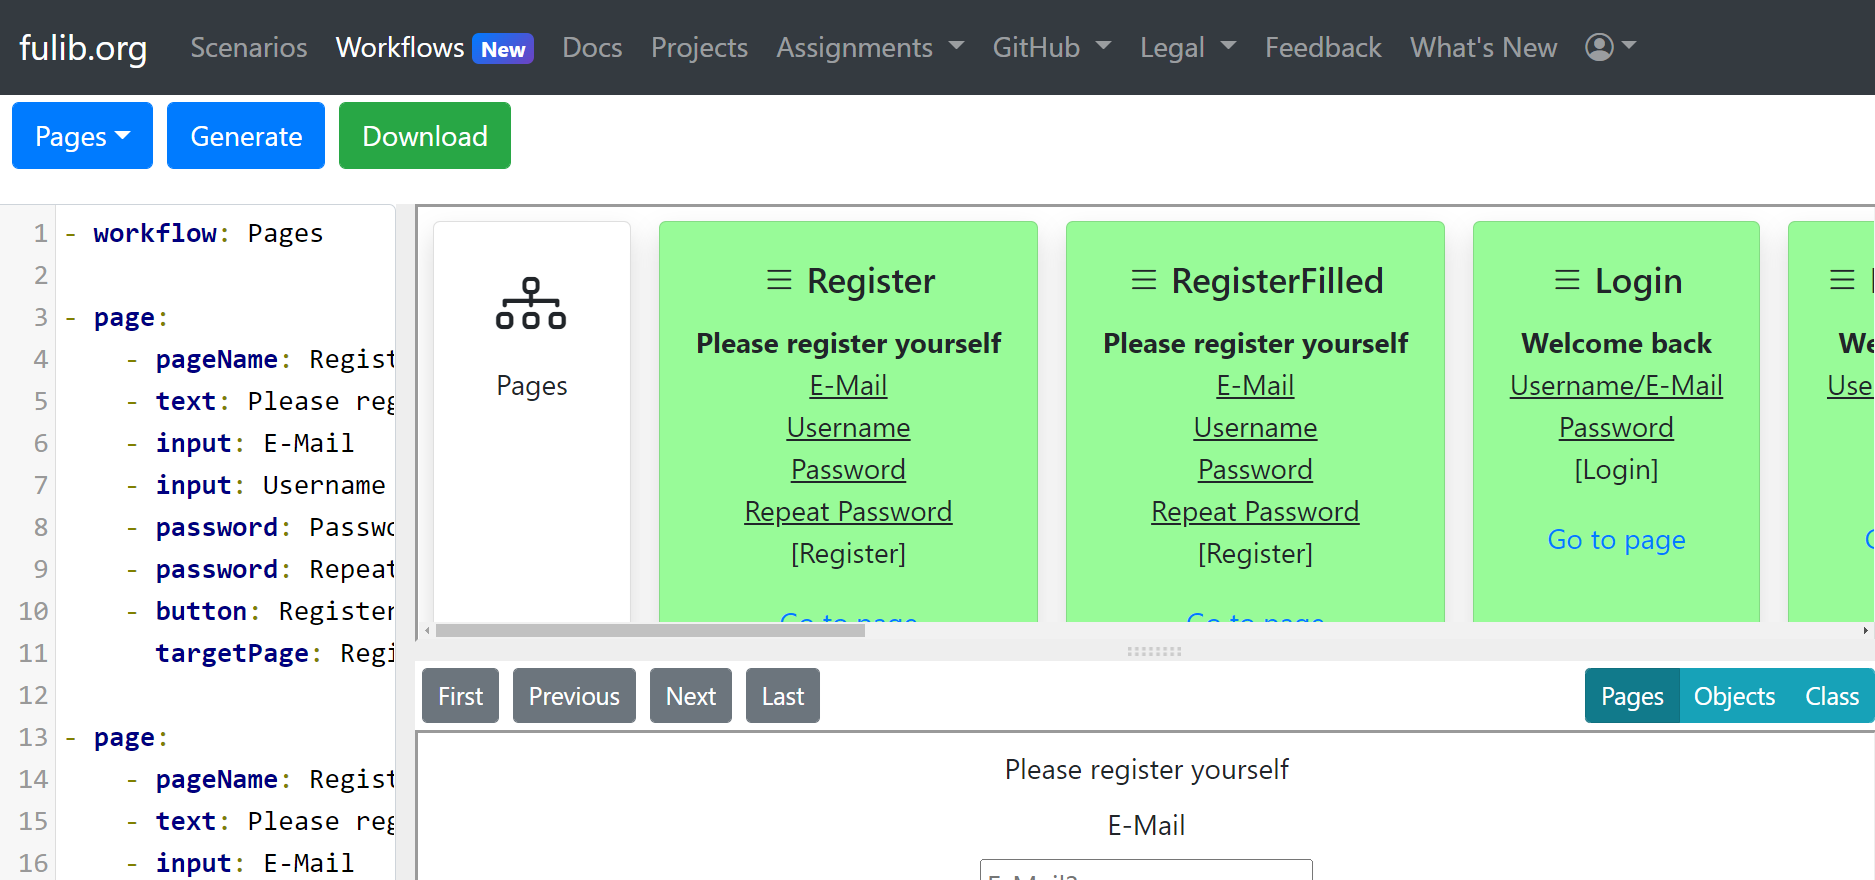
\includegraphics[width=0.75\textwidth]{images/5/fulibDotOrg}
    \caption{Aktueller Integrationsstand fulib.org}
    \label{fig:fulibDotOrg}
\end{figure}

Wie in Kapitel~\ref{subsec:fulibworkflows-web-editor} erwähnt, verläuft die Integration durch die zuvor gewählten Technologien gut.
Die Oberfläche und fast alle Funktionen konnten bereits übernommen werden.
Dennoch sind weitere Änderungen nötig, bevor der Web-Editor für fulibWorkflows für die Öffentlichkeit bereitgestellt werden kann.
